\chapter{Latome Hardware Design}\label{ch:latome-firmware}
% \parskip4pt \parindent12pt

\section{Specifications}\label{sec:specifications}
\subsection{The Liquid Argon Calorimeter Data Path}\label{sec:lar}
The LAr Calorimeter is made of 180,000 cells which are then summed up to form 34,048 supercells. The 12-bit readings of 8 supercells are serialized into one packet and sent through one optic fiber. The 116 LATOME boards are each connected to 48 optic fibers, thus receiving data from \(48\times8=384\) supercells. These boards are responsible for transforming the ADC levels into energy levels, reorganizing the data and summing some energies for LATOMEs covering specific regions of the detector and distributing the data to the Feature Extraction (FEX) system. The FEX system is responsible for processing the data and sending it to the Level 1 Trigger system.
% TODO: Precise what kind of cells

The FEX system is made of 3 groups: the Global Feature Extractor (gFEX), the Jet Feature Extractor (jFEX) and the Electron Feature Extractor (eFEX). Within these groups, gFEX only contains one board which gets summed data from all LATOMEs, thus showing the lowest granularity but with one board covering the whole detector. Then the jFEX is made of 6 boards, each receiving data from 19 LATOMEs, and finally the eFEX, with the highest granularity, is made of 24 boards, each receiving data from 4 LATOMEs.

\subsection{The LATOME Specifications}\label{sec:latome-specifications}
The part of the LATOME firmware responsible for the conversion of ADC levels into energy levels is referred to as \textit{User Code} in the LAr group. This code is not owned by the LATOME HLS team. However, the team is responsible for the different data organization steps, also called mapping or remapping, and the summing of energies for LATOMEs in specific regions of the detector. Additionally, since the output energies are only encoded on 10 bits, it is necessary to compress the data from 12 to 10 bits via a Multi Linear Encoder (MLE).

Initially, the whole LATOME firmware was written in VHDL. The implementation of all the functionalities took over 8 years and still had timing violations. Because in the next runs of the LHC, the amount of energy and collision is expected to increase, the LATOME design should be optimized to leave space for other functionalities, and sustain the increase in data.

\section{Existing Designs}\label{sec:existing-design}

\subsection{Original VHDL Design}\label{sec:original-vhdl-design}
The original design is characterized by more clock domain crossings than the current one.

\begin{figure}
    \centering
    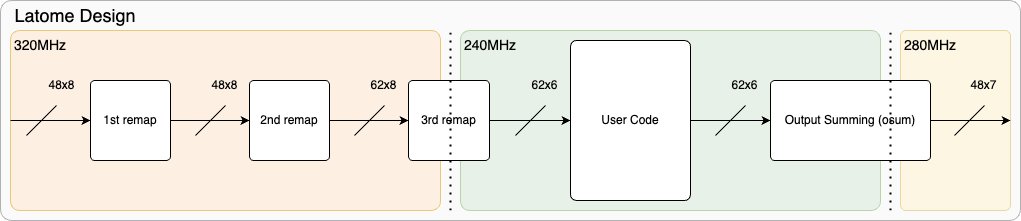
\includegraphics[width=1\textwidth]{latome_fw_vhdl.png}
    \caption{Original VHDL Design}
    \label{fig:original-vhdl-design}
\end{figure}

Because bunch crossings (BC) happen at a frequency of 40MHz, it is necessary to run the different blocks of the design at multiples of this frequency. The figure\ref{fig:original-vhdl-design} shows three different frequencies being used. At the first remap stage, since the frames are made of 8 words, it is necessary to run the blocks at 320MHz. Then the frames become 6 words long, corresponding to a frequency of 240MHz. Finally, the FEX systems expect 7 32 bits words, thus the frequency is 280MHz.

\begin{figure}[htb]
    \centering
    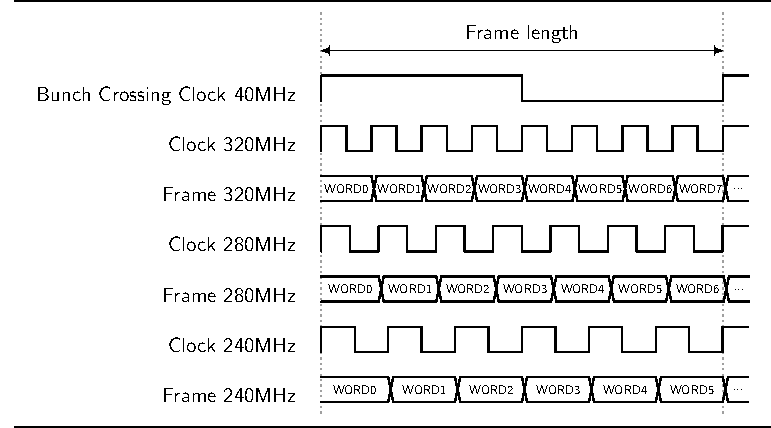
\includegraphics{timings/bc_clocks}
    \caption{Different clocks used in the design}
    \label{fig:bc-clocks}
\end{figure}

These clock domain crossings made the original implementation very complex...
%TODO: add more about the complexity of the original design

\subsection{Current HLS Design}\label{sec:current-hls-design}
When developing the new firmware from the specifications in HLS, very interesting insights from Dr. Marcos Oliveira emphasizing benefits of space division multiplexing were taken into account. By using parallel full frames, the frequency of the design blocks is not locked anymore depending on the frame size. This allows to reduce the logic dedicated only to synchronization and time-division multiplexing which can become very complex when there are dependencies between the words of the frame.

\begin{figure}
    \centering
    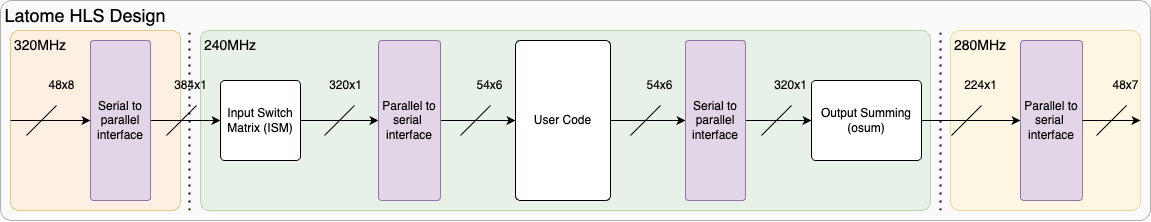
\includegraphics[width=1\textwidth]{latome_fw_hls.png}
    \caption{Current HLS Design}
    \label{fig:current-HLS-design}
\end{figure}

The figure \ref{fig:current-HLS-design} shows that all the remapping and processing blocks except for the User Code are being processed using parallel data. This is possible thanks to the serial-to-parallel and parallel-to-serial data transformation blocks. This approach drastically simplifies the design and showed very promising results in terms of area reduction, reduced latency.
% TODO: add more promising results